% Copyright (c) 2024, Francisco Fernandez
% License: CC BY-SA 4.0
%   https://github.com/fernandezfran/thesis/blob/main/LICENSE
\section{Energía, transporte y litio}

En la actualidad se utilizan distintas formas para generar energía y pueden 
dividirse en dos grandes tipos, las renovables y las no-renovables. Estas últimas
dominan la producción de energía mundial y están compuestas principalmente por 
combustibles fósiles y centrales nucleares, mientras que las energías renovables
abarcan más variantes como la biomasa, la hidráulica, la eólica y la solar, pero 
aún no son lo suficientemente utilizadas. Una de las particularidades de estas 
fuentes de energías renovables es su producción intermitente mientras que el 
consumo de la misma, independientemente de cómo se genere, es a demanda. Esto 
hace que sea necesario el involucramiento de vectores energéticos que permitan 
almacenar y transportar el excedente de energía que se genera en sus períodos de 
mayor producción para luego ser utilizada en los momentos de mayor demanda.

El sector del transporte terrestre, marítimo y aéreo es responsable de más de un 
tercio de las emisiones de CO$_2$ debido a su dependencia de los combustibles 
fósiles \cite{IEA}. Dicho esto, está claro que se debe fomentar opciones de desplazamiento menos intensivas
en carbono y con tecnologías más eficientes, como los vehículos eléctricos (EVs),
cuyos motores poseen una eficiencia para convertir la energía eléctrica en energía para las ruedas que ronda el 80\%, compárese este valor con las
eficiencias entre el 12\% y el 30\% de los motores a combustión interna para la misma tarea \cite{DOE}.

En los últimos años se ha producido un crecimiento exponencial en las ventas 
anuales de los EVs, como puede observarse en la Figura \ref{fig:evs}a \cite{EVV}. En la
última década, dichas ventas aumentaron aproximadamente un 500\% y se estima que
para la próxima década las ventas se multipliquen por 10. Estas ventas están 
concentradas en China y en algunos países y estados de Europa y Estados Unidos, 
respectivamente, debido a que en los países en desarrollo y emergentes influye 
negativamente su costo alto de adquisición y una falta de infraestructura para la 
recarga de sus baterías. En particular, durante el 2022 en Noruega el 79.3\% de 
los automóviles patentados fueron eléctricos. En el país que le sigue en la lista,
Suecia, se patentó un 32.1\% de EVs en dicho año \cite{PWC}.
\begin{figure}[h!]
    \centering
    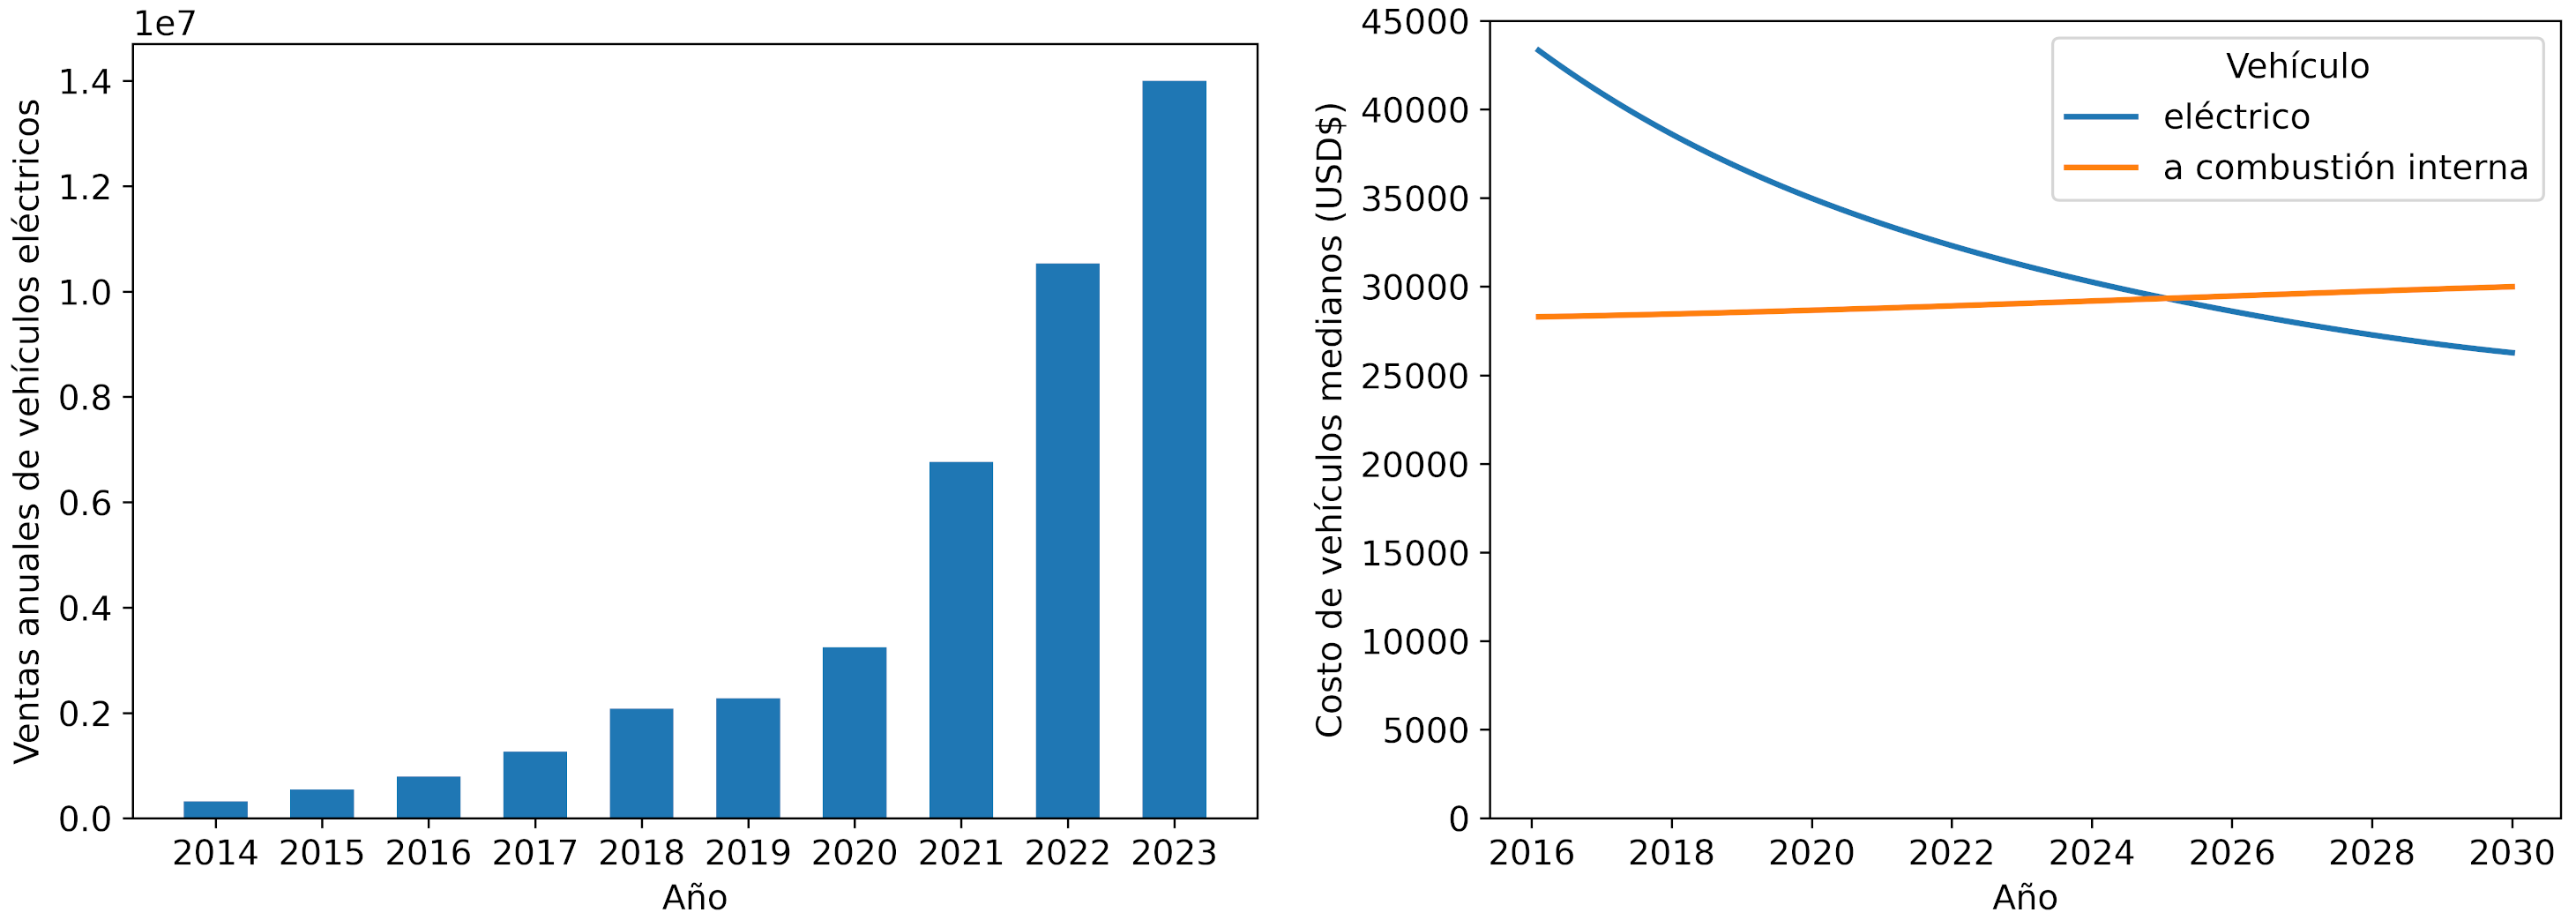
\includegraphics[width=\textwidth]{Introduccion/energia/evs.png}
    \caption{(a) Ventas anuales de vehículos eléctricos en la última década. Se 
    proyecta que para el 2030 las ventas asciendan a las 40 millones de unidades 
    frente a las 3 millones del año 2020 \cite{EVV}. (b) Proyección del costo en 
    dólares de vehículos eléctricos y de combustión interna en países 
    desarrollados \cite{BLOOMBERG}.}
    \label{fig:evs}
\end{figure}

En la Figura \ref{fig:evs}b se muestra la proyección en el costo de los vehículos 
eléctricos y de combustión interna realizada por la empresa financiera Bloomberg 
para los países desarrollados \cite{BLOOMBERG}. Se espera que para el año 2026 
los costos se igualen y que para el 2030 los EVs sean aproximadamente un 15\% más
baratos que los vehículos de combustión interna. Este cambio se debe a la 
disminución en el precio de la producción de baterías, que actualmente representa
aproximadamente el 40\% del costo del EV.

El sector energético en Argentina depende altamente de la utilización de 
combustibles fósiles, donde la generación de energía está dominada por el gas 
natural (65\%) y le siguen las centrales hidroeléctricas (18\%), plantas nucleares
(8\%), parques eólicos (7\%) y solares (1\%) \cite{IEA}. En cuanto al potencial de 
producción de fuentes renovables, Argentina tiene una gran capacidad, en sus 
fuentes eólicas y solares, por desarrollar. Además, es el cuarto productor mundial más 
grande de litio, que es un mineral crítico para la manufactura de sistemas de 
almacenamiento y transporte de energía, claves para la transición energética. 
El mismo representa el 7\% de la demanda de minerales críticos para vehículos eléctricos mientras que 
para almacenamiento en la red el porcentaje es del 10\%. Otros metales y 
minerales críticos se encuentran en la región de América Latina; por ejemplo, 
Paraguay posee la reserva más grande del mundo de titanio, Chile es el mayor 
productor de cobre, Brasil tiene las segundas reservas más grande de níquel y
hierro, las terceras de grafito y manganeso, la cuarta de aluminio y la quinta de 
fósforo, por último, Cuba se encuentra en el tercer puesto de reservas de cobalto.

En la Figura \ref{fig:iea-Li} se muestra la proyección en la demanda total de 
litio por año y por aplicación, donde la mayor contribución se encuentra para la 
utilización del mismo en vehículos eléctricos, mientras que una menor contribución 
se espera en aplicaciones de sistemas de almacenamiento estacionarios y otras 
aplicaciones que incluyen dispositivos electrónicos, medicamentos, lubricantes, 
entre otras \cite{IEA}. \todo{Este aumento de la demanda total de litio para los próximos años también se observa en el resto de los metales y minerales críticos presentes en las distintas componentes de las baterías \cite{IEA}.}
Cabe destacar que para el almacenamiento estacionario 
las baterías de ion-litio es muy probable que compitan con baterías de sodio o magnesio, entre 
otras. En el histograma de la Figura \ref{fig:iea-Li} pueden diferenciarse dos 
regiones, la primera de ellas entre los años 2022 y 2035, donde los aumentos
porcentuales de la demanda de litio con respecto a 5 años atrás son del 74\%, 
99\% y 76\%. Luego, desde el año 2035 al 2040, el cambio se encuentra en el 32\% y
dicho aumento porcentual continúa disminuyendo al 10\% y al 3\% en los períodos 
subsiguientes.
\begin{figure}[h!]
    \centering
    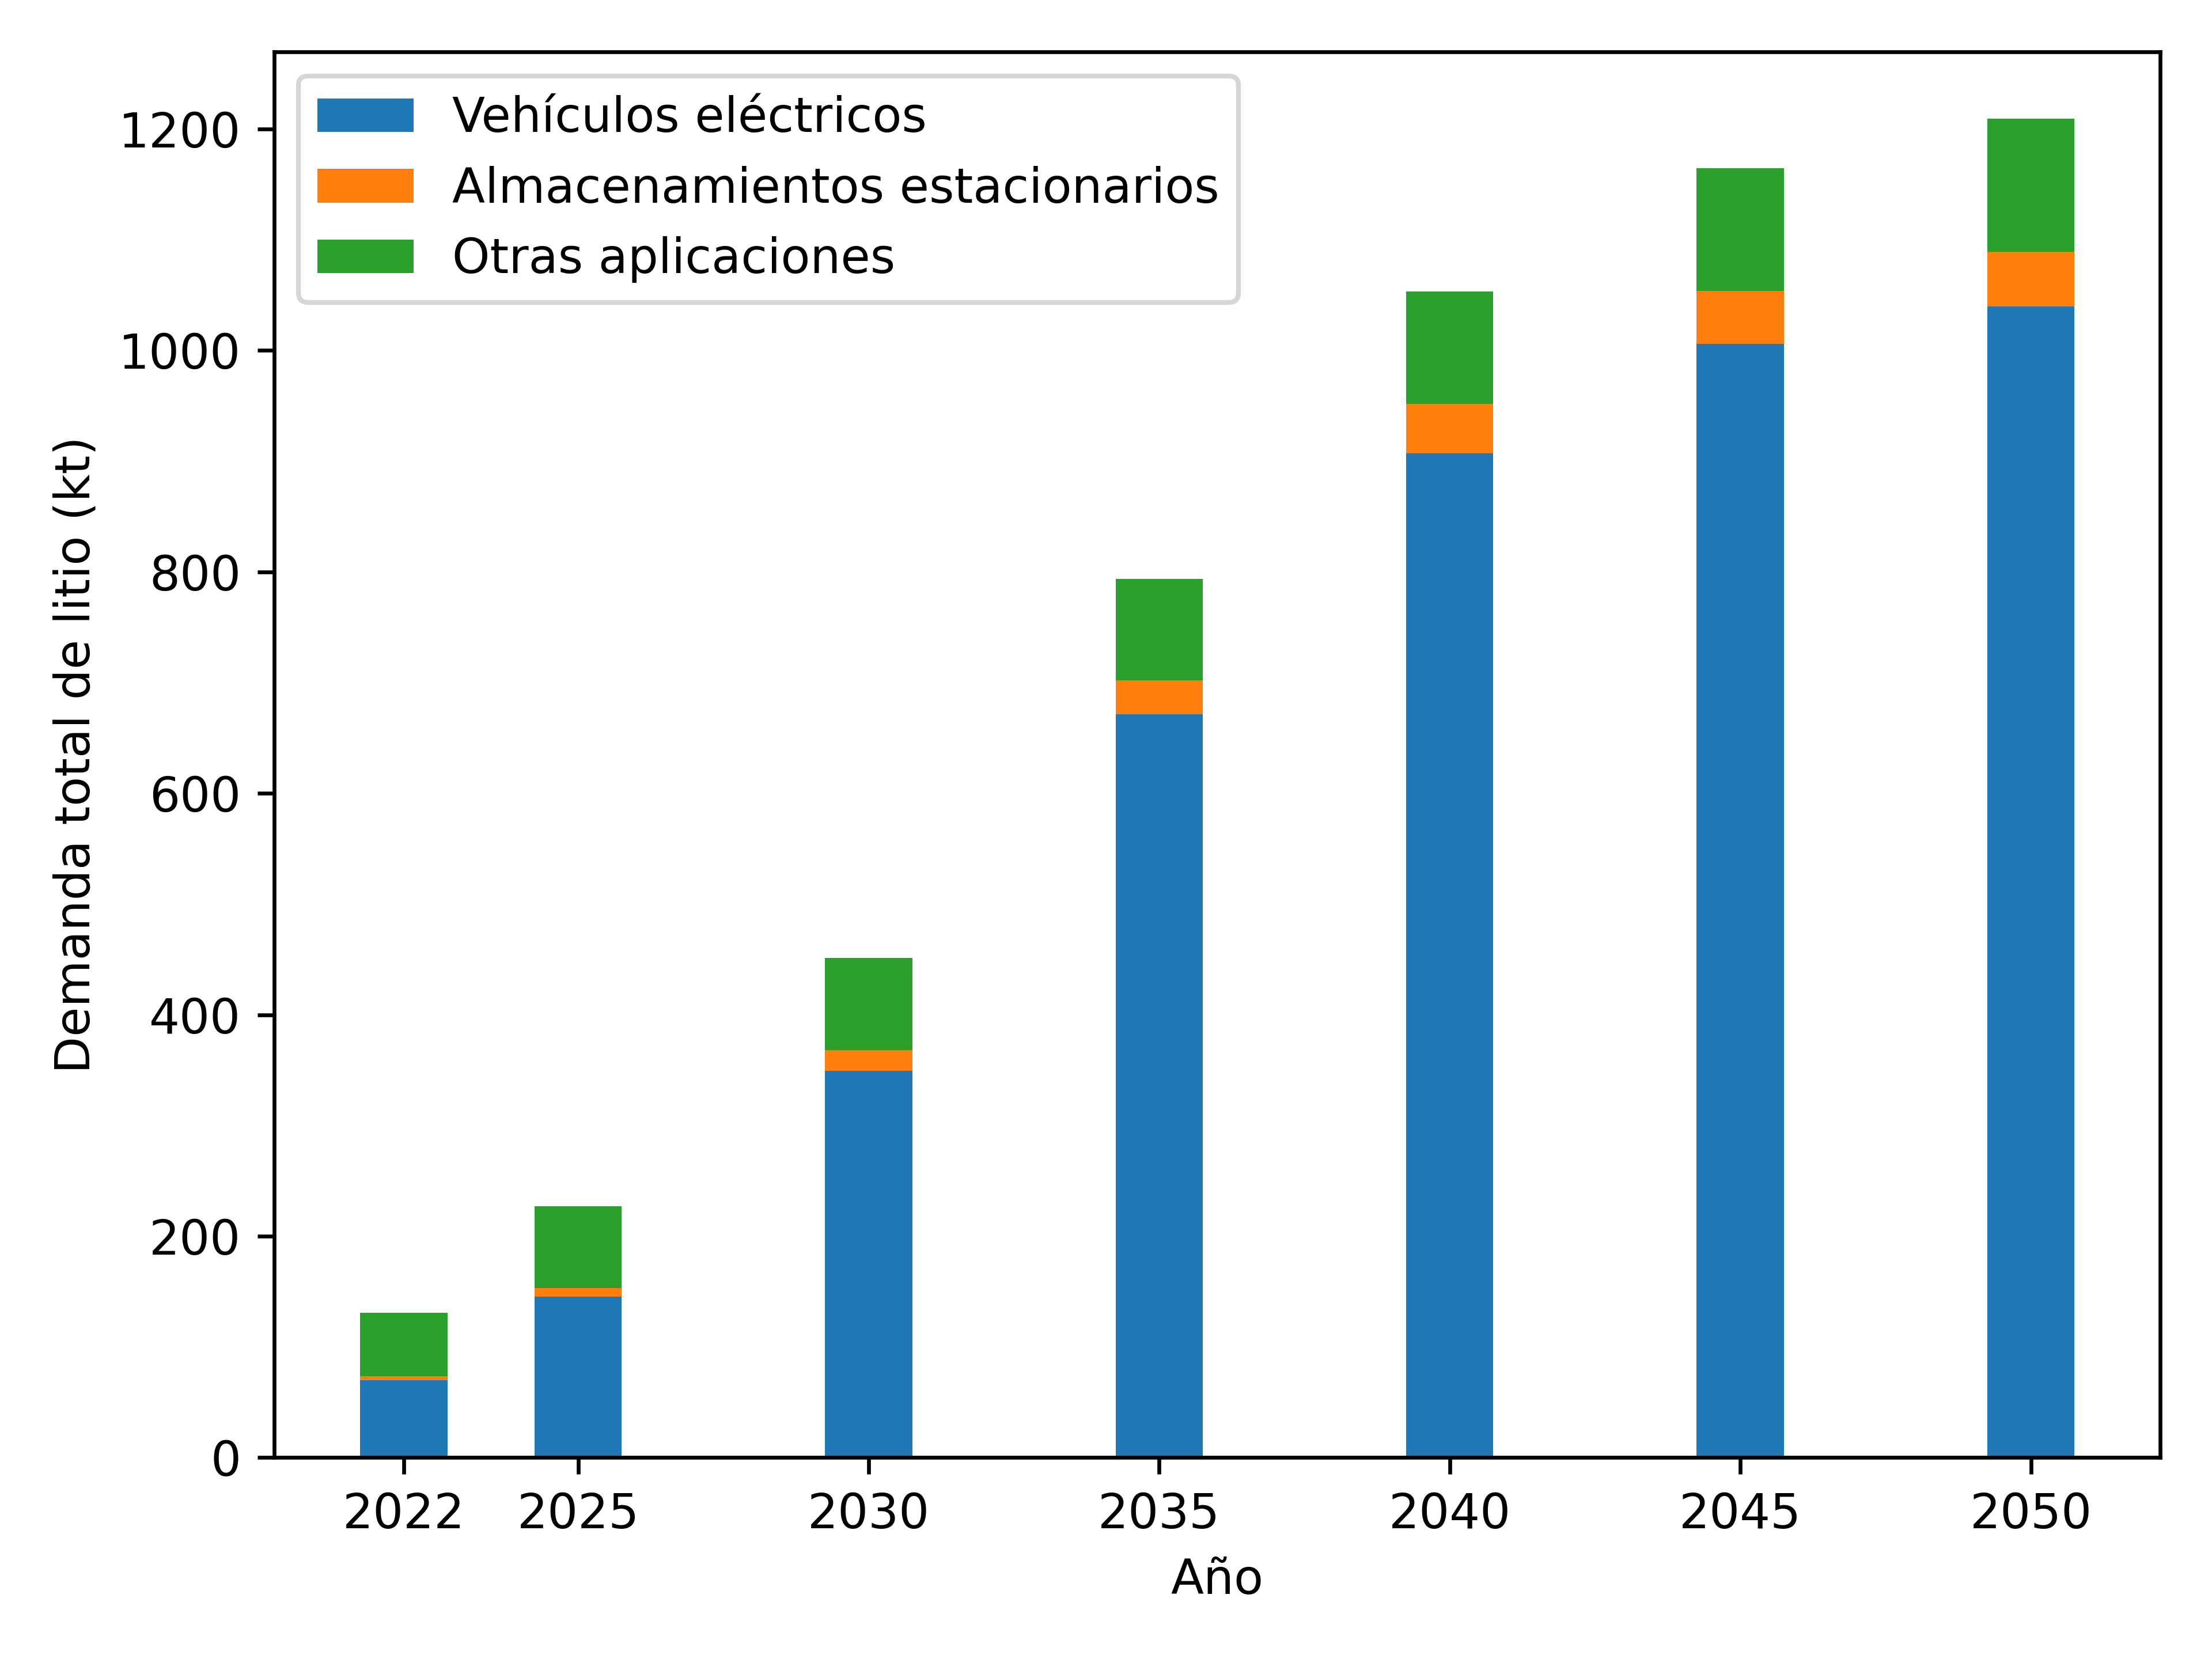
\includegraphics[width=.8\textwidth]{Introduccion/energia/iea-Li.png}
    \caption{Proyección de la demanda total de litio en kilotoneladas para el 
    período 2025-2050 para sus distintas aplicaciones: vehículos eléctricos (en 
    azul), sistemas de almacenamiento de energía estacionarios (en naranja) y
    otras aplicaciones (en verde). Fuente: \cite{IEA}.}
    \label{fig:iea-Li}
\end{figure}
